In this module you will learn
\begin{itemize}
	\item how to model physical phenomena to obtain second-order ODEs
\end{itemize}

\hfill \\


Whenever we model the movement of objects, we often find ourselves using \emph{Newton's Second Law of motion}:

\begin{definition}[Newton's Second Law of Motion]
	$F = m \cdot a$, \quad
	where $a$ is the acceleration of the object, $m$ is its mass, and $F$ is the net force acting on the object.
\end{definition}

Because this ``Law'' includes the acceleration of the object, and we know that
$$
{\rm acceleration} = a = \frac{d\,({\rm velocity})}{dt} = \frac{d\,v}{dt} = \frac{d^2 \, ({\rm position})}{dt^2} = \frac{d^2\,r}{dt^2},
$$
we will often end up with a Second-Order ODE.

Just like we did in module \ref{ODE:model}, we will follow the step by step procedure developed in chapter 1.

\paragraph{\emph{Step 1.}} Define the problem

\begin{example}

\begin{minipage}{.75\textwidth}
We want to model the position of an object attached to the end of a spring. \\

The first step is to decide on what we want to find at the end of the process. 
So we define:
\begin{itemize}
	\item $y(t) =$ the vertical position of the mass, where $y=0$ is the position of the mass at rest.
\end{itemize}
\end{minipage}
\hfill
\begin{minipage}{44pt}
\includegraphics*[height=100pt]{images/module16-spring-mass-dashpot.pdf}	
\end{minipage}
\end{example}


\paragraph{\emph{Step 2.}} Build a mind map

\begin{example}
We start with the mass and then we brainstorm about the things that affect the mass:
\begin{center}
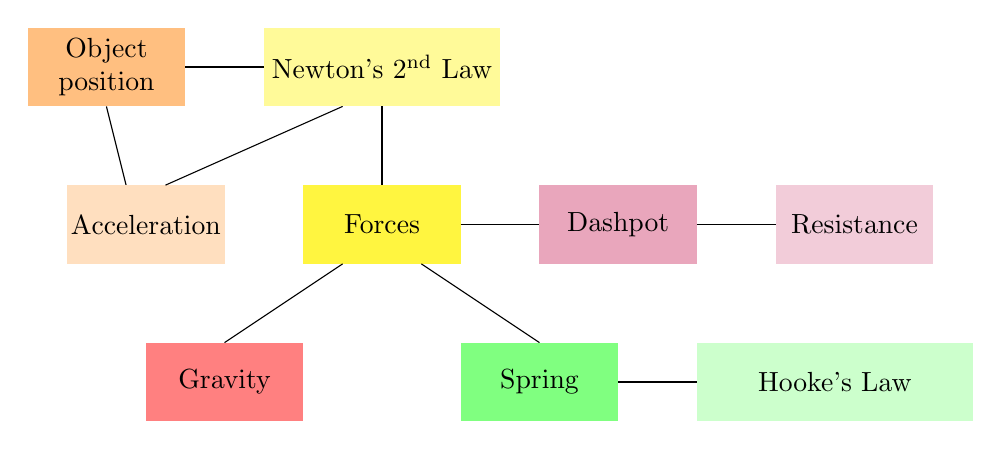
\begin{tikzpicture}
    \fill[color=orange!50!white] (-4.5,2) rectangle (-2.5,3) node[pos=.5,text width=1.5cm,align=center] {\color{black}Object position};
    \draw (-3.5,2) -- (-3.25,1);
    \fill[color=orange!25!white] (-4,1) rectangle (-2,0) node[pos=.5] {\color{black}Acceleration};
    \draw (-0.5,2) -- (-2.75,1);
    \draw (-2.5,2.5) -- (-1.5,2.5);
    \fill[color=yellow!40!white] (-1.5,2) rectangle (1.5,3) node[pos=.5] {\color{black}Newton's $2^{\rm nd}$ Law};
    \draw (0,1) -- (0,2);
  \fill[color=yellow!75!white] (-1,0) rectangle (1,1) node[pos=.5] {\color{black}Forces};
    \draw (-0.5,0) -- (-2,-1);
    \fill[color=red!50!white] (-1,-1) rectangle (-3,-2) node[pos=.5] {\color{black}Gravity};
    \draw (0.5,0) -- (2,-1);
    \fill[color=green!50!white] (3,-2) rectangle (1,-1) node[pos=.5] {\color{black}Spring};
    \draw (3,-1.5) -- (4,-1.5);
    \fill[color=green!20!white] (4,-2) rectangle (7.5,-1) node[pos=.5] {\color{black}Hooke's Law};
    \draw (1,0.5) -- (2,0.5);
    \fill[color=purple!35!white] (2,0) rectangle (4,1) node[pos=.5] {\color{black}Dashpot};  
    \draw (4,0.5) -- (5,0.5);
    \fill[color=purple!20!white] (5,0) rectangle (7,1) node[pos=.5] {\color{black}Resistance};  
\end{tikzpicture}
\end{center}
	
\end{example}


\paragraph{\emph{Step 3.}} Make assumptions

\begin{example}
In this step, we discuss the mind map we created and how we plan to address each of the boxes, or only some of the boxes. This will involve making assumptions and providing an explanation to the assumptions we make.

\begin{enumerate}
	\item As we described before the example, the plan is to use Newton's Second Law of Motion to describe the motion of the mass. This involves three quantities:
	\begin{itemize}
		\item mass: we assume that this is known to the modeller;
		\item acceleration: as we mentioned above, this is directly related to the position of the object. We have $y''(t)=$ acceleration, as long as we are assuming that the object is moving only vertically;
		\item forces: we need to find all the forces acting on the object and add them.
	\end{itemize}
\end{enumerate}

The forces acting on the object need to be discussed separately:
\begin{itemize}
	\item Gravity: we will go on a limb here and say that the force of the spring is much larger, so we will ignore this force;
	\item Spring: the force of the spring that acts on the mass follows Hooke's Law that says that the force is proportional to the extension/contraction of the spring. The constant of proportionality depends on the spring and we assume that it is known;
	\item Dashpot: the dashpot provides resistance. We will assume that it provides linear resistance to movement: the force is proportional to the velocity, with a proportionality constant that depends on the dashpot and is assumed to be known to the modeller.
\end{itemize}
	
\end{example}


\paragraph{\emph{Step 4.}} Construct a model

\begin{example}
We will start with Newton's Second Law of motion:
\begin{itemize}
	\item $m y''(t) = F(t)$ \\
\end{itemize}

and we will  add the different forces one by one:
\begin{itemize}
	\item Spring: the force of the spring is \quad $- k y(t)$; \hfill (you should check that the sign makes sense)
	\item Dashpot: the force of the dashpot is \quad $- \gamma y'(t)$. \hfill (you should also check the sign of this term) \\
\end{itemize}

Right now we have the following model:
$$
m y''(t) = -ky(t) - \gamma y'(t).
$$

\end{example}


\paragraph{\emph{Step 5.}} Model assessment

We'll skip this part here, but you should try to develop some tests to check the validity of the model we came up with.
Specifically, the fact that we ignored gravity should be checked to make sure that it doesn't affect our model too much.

%\paragraph{\emph{Step 6.}} Putting it all together in a report
%
%We'll skip this part here.




